\documentclass[10pt,pdf]{beamer}
\mode<presentation>
%http://www.hartwork.org/beamer-theme-matrix/
\usetheme{Warsaw}
\usecolortheme{whale}
\setbeamerfont{frametitle}{size=\small}

% \usepackage[utf8]{inputenc}
% \usepackage[T2A]{fontenc}
% \usepackage[russian,english]{babel}

\usepackage{amssymb}
\usepackage{amsmath}
\usepackage{graphicx}
\graphicspath{{images/}}
\usepackage[font=scriptsize]{subfig}
%\usepackage{epstopdf}
\usepackage[english]{isodate}
%\usepackage[noend]{algorithmic}
%\usepackage{algorithm}
%\usepackage{multirow}
\usepackage{tikz}
%\usepackage{pgfplots}
\usepackage{hyperref}
%\usepackage{tabulary}
\usepackage[utf8]{inputenc}

\defbeamertemplate{description item}{align left}{\insertdescriptionitem\hfill}

\usetikzlibrary{decorations.pathreplacing}
\newcommand{\tikzmark}[2]{\tikz[remember picture,baseline=(#1.base)]{\node[inner sep=0pt] (#1) {#2};}}

%\algsetup{indent=2em,linenosize=\footnotesize}

\title{Automatic Mobile Video Director}
\author[Alexander Egurnov \and Thilo Weigold \and Jon Pettersen \and Alf-André Walla]{
	\texorpdfstring{
		\begin{columns}
			\column{.45\linewidth}
			\centering
			{Alexander Egurnov\inst{\dagger}\\
			\href{mailto:aegurnov@mail.uni-mannheim.de}{aegurnov@mail.uni-mannheim.de}}
			\column{.45\linewidth}
			\centering
			{Thilo Weigold\inst{\dagger}\\
			\href{mailto:tweigold@mail.uni-mannheim.de}{tweigold@mail.uni-mannheim.de}}
		\end{columns}
		\vspace{0.5cm}
		\begin{columns}
			\column{.45\linewidth}
			\centering
			{Jon Pettersen\inst{*}\\
			\href{mailto:jonup@student.matnat.uio.no}{jonup@student.matnat.uio.no}}
			\column{.45\linewidth}
			\centering
			{Alf-André Walla\inst{*}\\
			\href{mailto:alfandrw@ifi.uio.no}{alfandrw@ifi.uio.no}}
		\end{columns}
	}
	{Alexander Egurnov, Thilo Weigold, Jon Pettersen, Alf-André Walla}
}
\institute[University of Mannheim]{
	\inst{\dagger} University of Mannheim \and %
	\inst{*} University of Oslo}
%\institute[University of Mannheim]{University of Mannheim}

\begin{document}

% \AtBeginSection[]
% {
%     \begin{frame}
%         \frametitle{Table of Contents}
%         \tableofcontents[currentsection]
%     \end{frame}
% }

% \AtBeginSubsection[]
% {
%     \begin{frame}
%         \frametitle{Table of Contents}
%         \tableofcontents[currentsection, currentsubsection]
%     \end{frame}
% }
\setcounter{framenumber}{0}
\setbeamertemplate{footline}
{
  \leavevmode%
  \hbox{%
  \begin{beamercolorbox}[wd=.3\paperwidth,ht=2.25ex,dp=1ex,center]{title in head/foot}%
	\usebeamerfont{title in head/foot}\insertshorttitle
  \end{beamercolorbox}%
  \begin{beamercolorbox}[wd=.5\paperwidth,ht=2.25ex,dp=1ex,center]{author in head/foot}%
	\usebeamerfont{author in head/foot}\insertshortauthor
  \end{beamercolorbox}%
  \begin{beamercolorbox}[wd=.2\paperwidth,ht=2.25ex,dp=1ex,right]{date in head/foot}%
	\insertframenumber{} / \inserttotalframenumber\hspace*{2ex} 
  \end{beamercolorbox}}%
  \vskip0pt%
}

\begin{frame}
	\titlepage
\end{frame}

\begin{frame}
	\frametitle{Content}
	\tableofcontents
\end{frame}

\section{Introduction}
\begin{frame}
	\frametitle{Motivation}
	What we wanted to build
\end{frame}

\begin{frame}
	\frametitle{Related work}
	What other people have build before us
\end{frame}

\section{Software}

	\subsection{System Overview}
	\begin{frame}
		\frametitle{General system overview}
		\begin{figure}[!t]
			\centering
			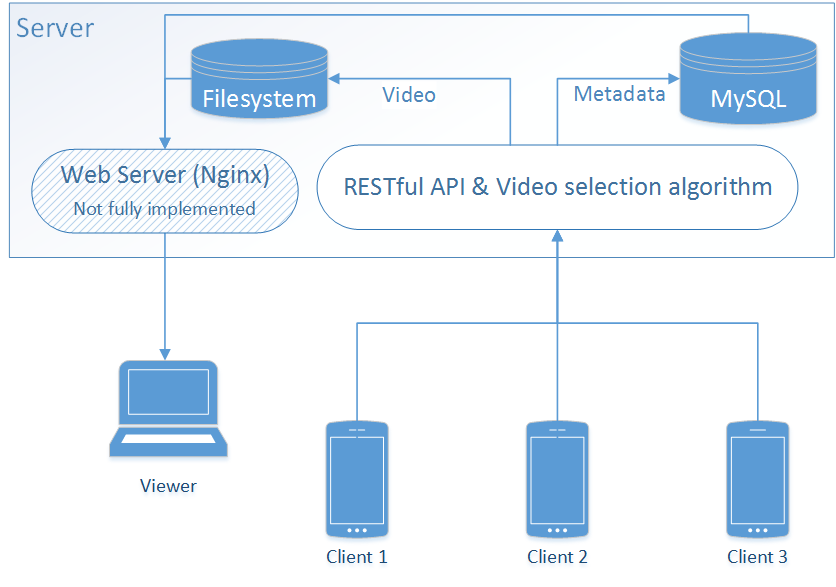
\includegraphics[width=\textwidth,height=.9\textheight,keepaspectratio]{sys_arch.png}
			\label{fig:gen_arch}
		\end{figure}
	\end{frame}

	\subsection{Client application}
	\begin{frame}	
	\frametitle{HTTP connection}
	\begin{columns}[t]
		\begin{column}[t]{0.5\linewidth}
			Http client:
			\begin{itemize}
				\item HttpURLConnection
				\item HttpAsnycTask class to run network operations independently from UI thread
				\item Implementation of an Android service to check requested video uploads
			\end{itemize}
		\end{column}
		\begin{column}[t]{0.5\linewidth}
			Class diagram:
			\begin{itemize}
				\item ...
			\end{itemize}
			
		\end{column}		
	\end{columns}	
\end{frame}

\begin{frame}	
	\frametitle{Camera}
	\begin{columns}[t]
		\begin{column}[t]{0.5\linewidth}
			Camera:
			\begin{itemize}
				\item No use of phone's default camera application.
				\item Own CameraActivity
				\item Use of Android's MediaRecorder.
				\item Storage of video files (.mp4 format) in the public directory for further usage. 
			\end{itemize}
		\end{column}
		\begin{column}[t]{0.5\linewidth}
			Class diagram:
			\begin{itemize}
				\item 
			\end{itemize}
			
		\end{column}		
	\end{columns}	
\end{frame}

\begin{frame}	
	\frametitle{Sensors}
	\begin{columns}[t]
		\begin{column}[t]{0.5\linewidth}
			Camera:
			\begin{itemize}
				\item Use of the accelerometer sensor
				\item Shake Detection
				\item Tilt Detection
				\item Preprocessed sensor data: ”Counter” value is send to the server.
				\item easy to add new sensors
			\end{itemize}
		\end{column}
		\begin{column}[t]{0.5\linewidth}
			Class diagram (Observer pattern): 
			\begin{itemize}
				\item ...
			\end{itemize}
			
		\end{column}		
	\end{columns}	
\end{frame}

\begin{frame}	
	\frametitle{SQLite database}
	SQLite database:
		\begin{itemize}
			\item Problem: coupling of actual video file and meta data persistently. 
			\item Use of Android's SQLite databases to have meta data persistently.
			\item Table: metadata
			\item Each filename is unique -> column filename be handled as a foreign key to the actual video file.
		\end{itemize}
\end{frame}

\begin{frame}	
	\frametitle{SQLite database}
		\begin{itemize}
			Table metadata: \hrule
			\begin{description}	
				\item[id] int primary key
				\item[filename] text
				\item[timestamp] text
				\item[duration] int
				\item[width] int
				\item[height] int
				\item[shaking] int
				\item[tilt] int
				\item[serverId] int
				\item[status] int
			\end{description}
		\end{itemize}
\end{frame}

\begin{frame}	
	\frametitle{User interface}
	\begin{columns}[t]
		\begin{column}[c]{.5\textwidth}
			\begin{figure}[!t]
				\centering
				\subfloat[Main]{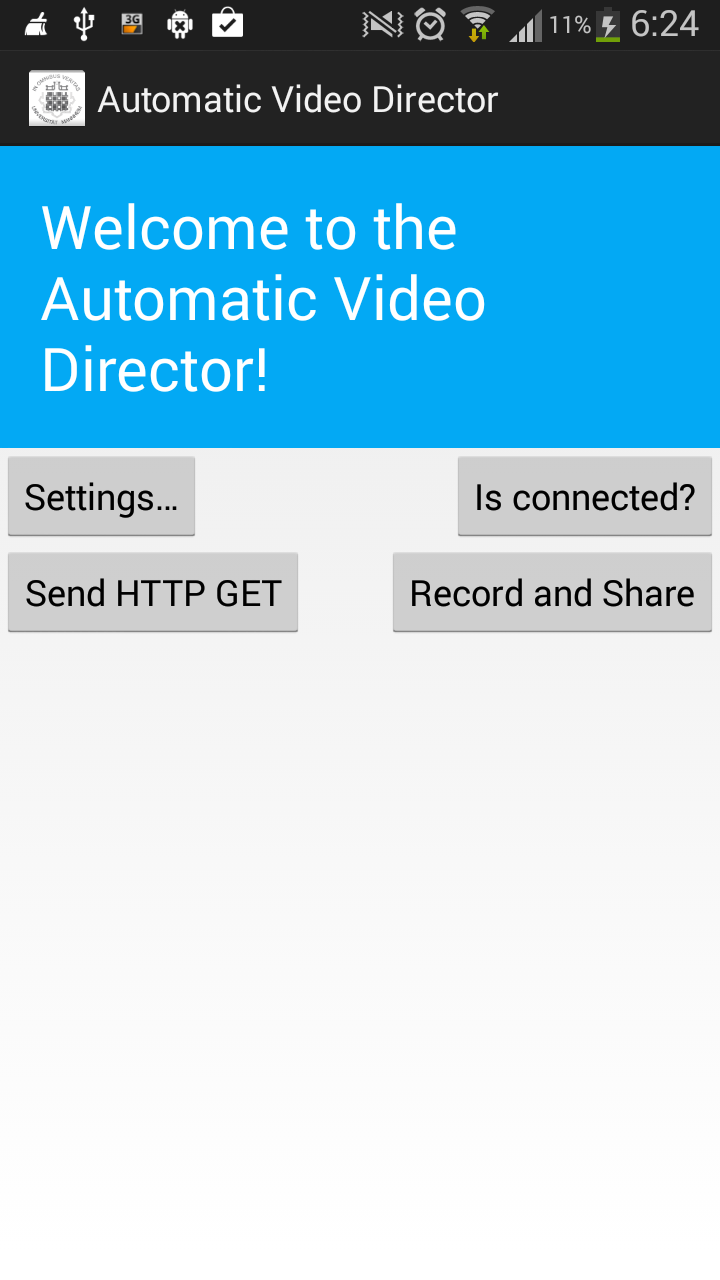
\includegraphics
						[width=.49\textwidth,height=.9\textheight,keepaspectratio]
						{ui_main.png}%
					\label{fig:ui_main}}
				\hfill
				\subfloat[Settings]{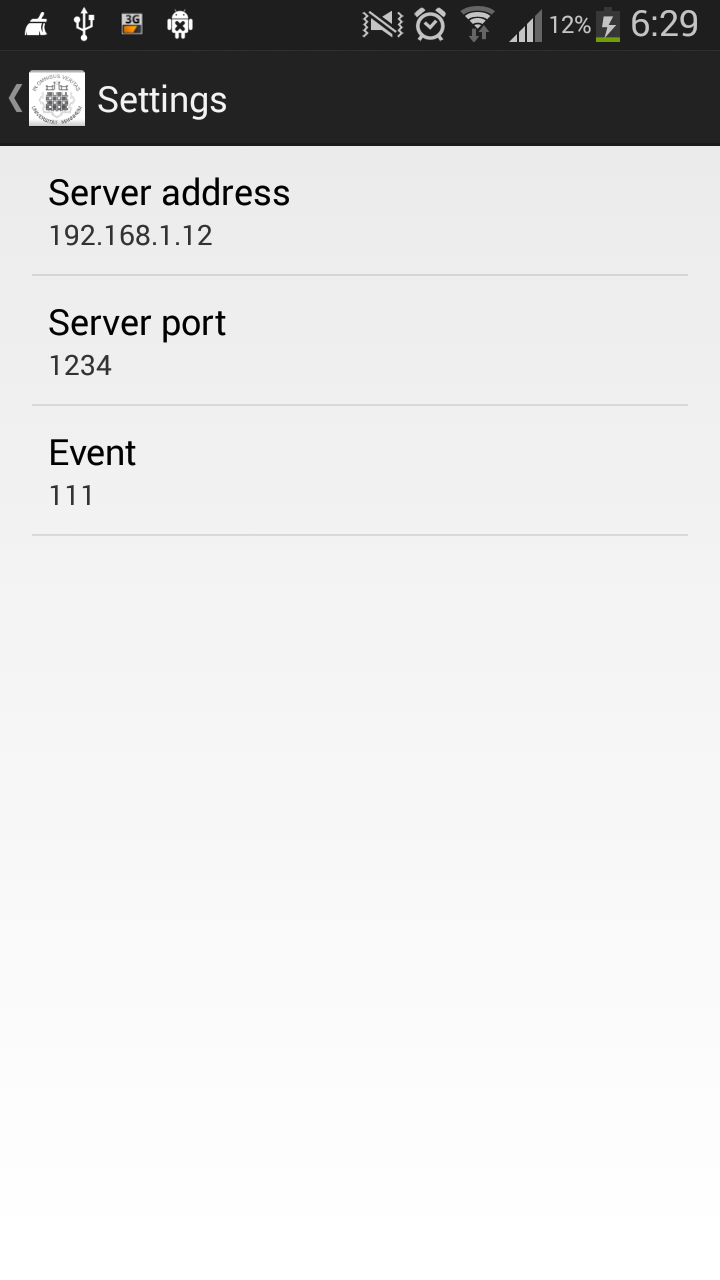
\includegraphics
					[width=.49\textwidth,height=.9\textheight,keepaspectratio]
					{ui_interface.png}%
					\label{fig:ui_settings}}
				\label{fig:ui_menu}
			\end{figure}
		\end{column}
		\begin{column}[c]{.5\textwidth}
			\begin{figure}[!t]
				\centering
				\subfloat[Camera]{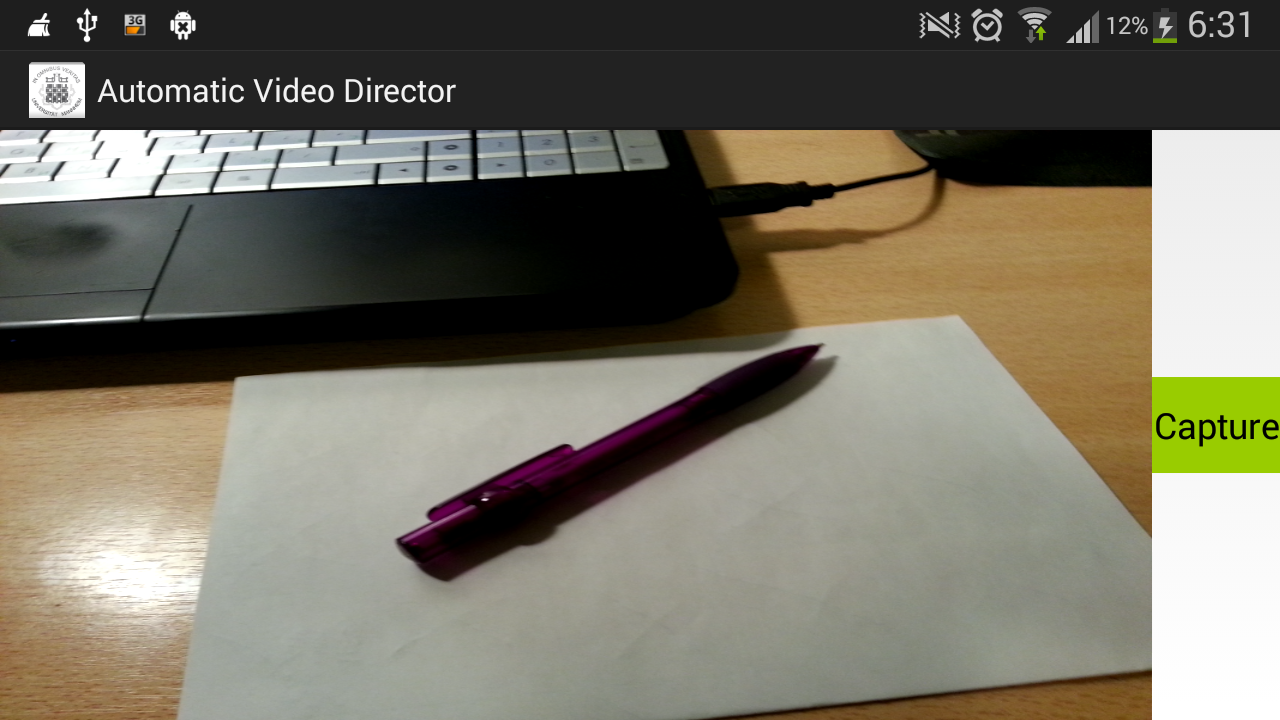
\includegraphics
					[width=\textwidth,height=.3\textheight,keepaspectratio]
					{ui_cam_green.png}%
					\label{fig:ui_cam_green}}
				\vfill
				\subfloat[Metadata upload]{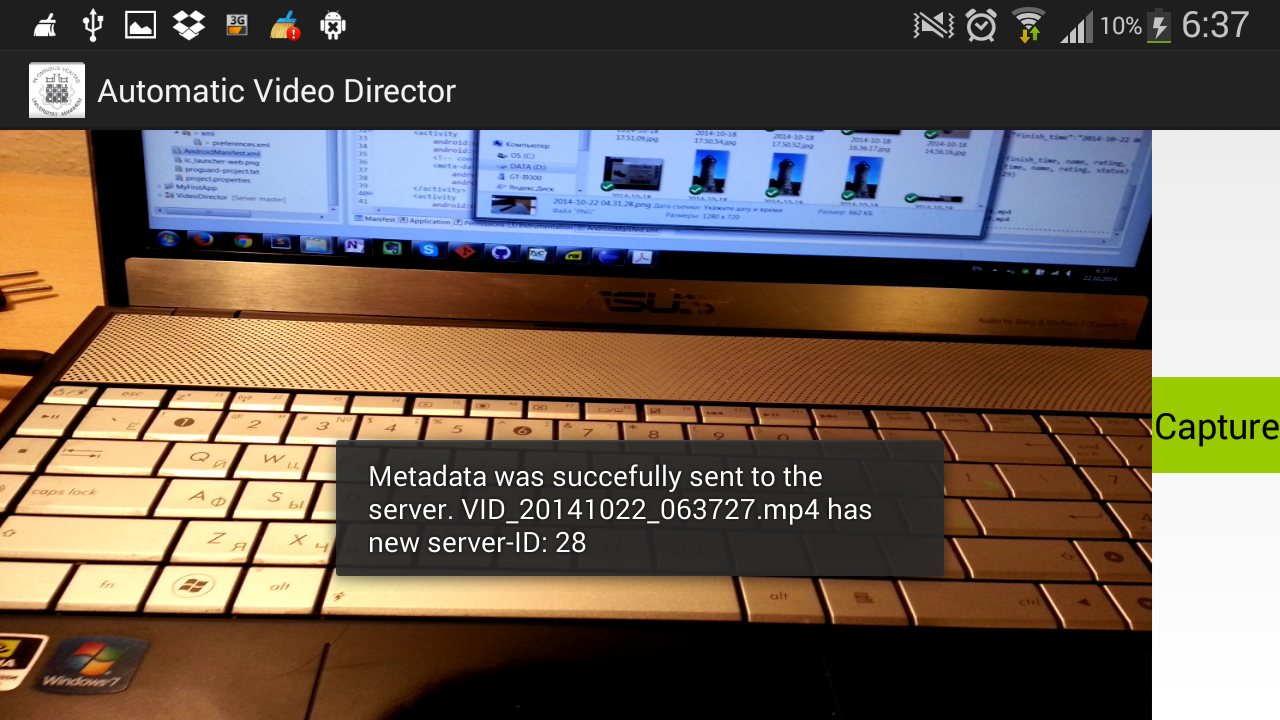
\includegraphics
					[width=\textwidth,height=.3\textheight,keepaspectratio]
					{ui_metadata.png}%
					\label{fig:ui_metadata}}
				\label{fig:ui_cam}
			\end{figure}
		\end{column}
	\end{columns}
\end{frame}

	\subsection{Server application}
	\begin{frame}	
	\begin{columns}[t]
		\begin{column}[t]{0.5\linewidth}
			Application:
			\begin{itemize}
				\item Java 8
				\item Spark Web Framework\footnotemark[1]
				\item Gson\footnotemark[2]
				\item Maven\footnotemark[3]
			\end{itemize}
		\end{column}
		\begin{column}[t]{0.5\linewidth}
			Database:
			\begin{itemize}
				\item MySQL
			\end{itemize}
			
			Web Interface:
			\begin{itemize}
				\item Nginx web server\footnotemark[4]
				\item nginx-rtmp-module\footnotemark[5]
				\item JWplayer\footnotemark[6] or Video.js\footnotemark[7]
				\item HTML+JavaScript (temporary)
			\end{itemize}
		\end{column}		
	\end{columns}	
	
{\tiny
	\footnotetext[1]{\url{http://sparkjava.com/}}
	\footnotetext[2]{\url{https://code.google.com/p/google-gson/}}
	\footnotetext[3]{\url{http://maven.apache.org/}}
	\footnotetext[4]{\url{https://github.com/arut/nginx-rtmp-module}}
	\footnotetext[5]{\url{http://nginx.org/}}
	\footnotetext[6]{\url{http://www.jwplayer.com/}}
	\footnotetext[7]{\url{http://www.videojs.com/}}
}
\end{frame}

\begin{frame}	
	%\begin{columns}[t]
		%\begin{column}[t]{0.5\linewidth}
			Application:
			\begin{itemize}
				\item RESTful API
				\item Client sessions with cookies
				\item No registration needed
				\item Rating takes duration into account
			\end{itemize}
		%\end{column}
		%\begin{column}[t]{0.5\linewidth}
			%
		%\end{column}		
	%\end{columns}	
\end{frame}

\begin{frame}
	\frametitle{Database tables}
	\setbeamertemplate{description item}[align left]
	\begin{columns}[t]
		\begin{column}[t]{0.5\linewidth}
			event \hrule
			\begin{description}[name]
				\item[id] int primary key 
				\item[name] varchar(255) 
				\item[ts] timestamp
			\end{description}
			
			\vspace{0.5cm}
			event\_videos \hrule
			
			\begin{description}[event\_id]
				\item[event\_id] int %\tikzmark{E}
				\item[video\_id] int %\tikzmark{V}
			\end{description}
			%\begin{tikzpicture}[remember picture,overlay]
				%\draw[decorate,decoration={brace}] (E.north east) -- node[right] {primary key} (E.north east |- V.south east);
			%\end{tikzpicture}

		\end{column}
		\begin{column}[t]{0.5\linewidth}
			video \hrule
			\begin{description}[finish\_time]	
				\item[id] int primary key
				\item[finish\_time] timestamp
				\item[duration] int
				\item[width] int
				\item[height] int
				\item[shaking] int
				\item[tilt] int
				\item[name] varchar(255)
				\item[rating] int
				\item[status] int
			\end{description}
		\end{column}		
	\end{columns}	
\end{frame}

	\subsection{Client-server interaction}
	\begin{frame}	
	\frametitle{Client-server data exchange}
	\begin{figure}[!t]
		\centering
		\includegraphics[width=\textwidth,height=\textheight,keepaspectratio]{protocol_cr1.png}
		\label{fig:protocol1}
	\end{figure}
\end{frame}

\begin{frame}	
	\frametitle{Client-server data exchange (continued)}
	\begin{figure}[!t]
		\centering
		\includegraphics[width=\textwidth,height=\textheight,keepaspectratio]{protocol_cr2.png}
		\label{fig:protocol2}
	\end{figure}
\end{frame}

\begin{frame}	
	\frametitle{Protocol description}
	\small
	\setbeamertemplate{description item}[align left]
	\begin{description}[PUT /video/\textit{video\_id}]
		\item[GET /events]
			Lists all events (including videos) in~JSON.			
		\item[GET /event/\textit{id}]
			Returns Event (including videos) in~JSON.					
		\item[POST /event/new]
			Create new event from JSON.
			Expects request body to be a JSON string containing attribute~\textit{name}.			
		\item[POST /event/\textit{id}]
			Upload JSON metadata about a video for Event with given \textit{id}.			
		\item[PUT /video/\textit{video\_id}]
			Upload video~\textit{video\_id}.
			Expects request body to be a file stream containing a full video file.			
		\item[GET /video/\textit{video\_id}]
			Retrieve video~\textit{video\_id}.			
		\item[GET /selected]
			Retrieve a list of selected but not yet uploaded videos in JSON.			
	\end{description}
\end{frame}

	\subsection{Meta data format}
	\begin{frame}
	\frametitle{Metadata format}
	\setbeamertemplate{description item}[align left]
	\begin{description}[finish\_time]
		\item[id] 
			Server-side unique identification of the video.
		\item[name]
			File name in client's local file system.			
		\item[finish\_time]
			Video creation time in the format: yyyy-mm-dd hh:mm:ss
		\item[duration]
			Video duration in milliseconds.	
		\item[width]
			Video frame width in pixels.
		\item[height]
			Video frame height in pixels.		
		\item[shaking]
			Amount of shaking detected by sensors.
		\item[tilt]
			The amount of tilt holding of the camera.
		\item[status]
			Video status. Indicates video life cycle phase.
		\item[event\_id]
			Unique server-side identifier of an event.		
	\end{description}
\end{frame}

\begin{frame}[fragile]
	\frametitle{JSON vs. XML}
		\begin{itemize}
			\item JSON more lightweight then  XML, less overhead.
			\item Library org.json for Java for fast parsing.
			\item Serialization and deserialization in JSON more efficient then XML.
			\item Describes meta data properly, XML better used for data in the document paradigm
		\end{itemize}
\end{frame}

\begin{frame}[fragile]
	\frametitle{Metadata example (formatted) }
		HTTP\_POST /event/\textit{id}\footnotemark
		\begin{verbatim}
		{
		    "id":30,
		    "duration":3669,
		    "height":1080,
		    "shaking":0,
		    "tilt":24,
		    "width":1920,
		    "finish_time":"2014-11-05 14:01:12.0",
		    "name":"VID_20141105_140107.mp4"
		}
		\end{verbatim}
		\footnotetext{\textsl{event\_id} is transfered as a part of URL}
\end{frame}


\section{Video Director Algorithm}
\subsection{Video life cycle}
\begin{frame}[fragile]	
	\frametitle{Video life cycle}
	\begin{figure}[!t]
		\centering
		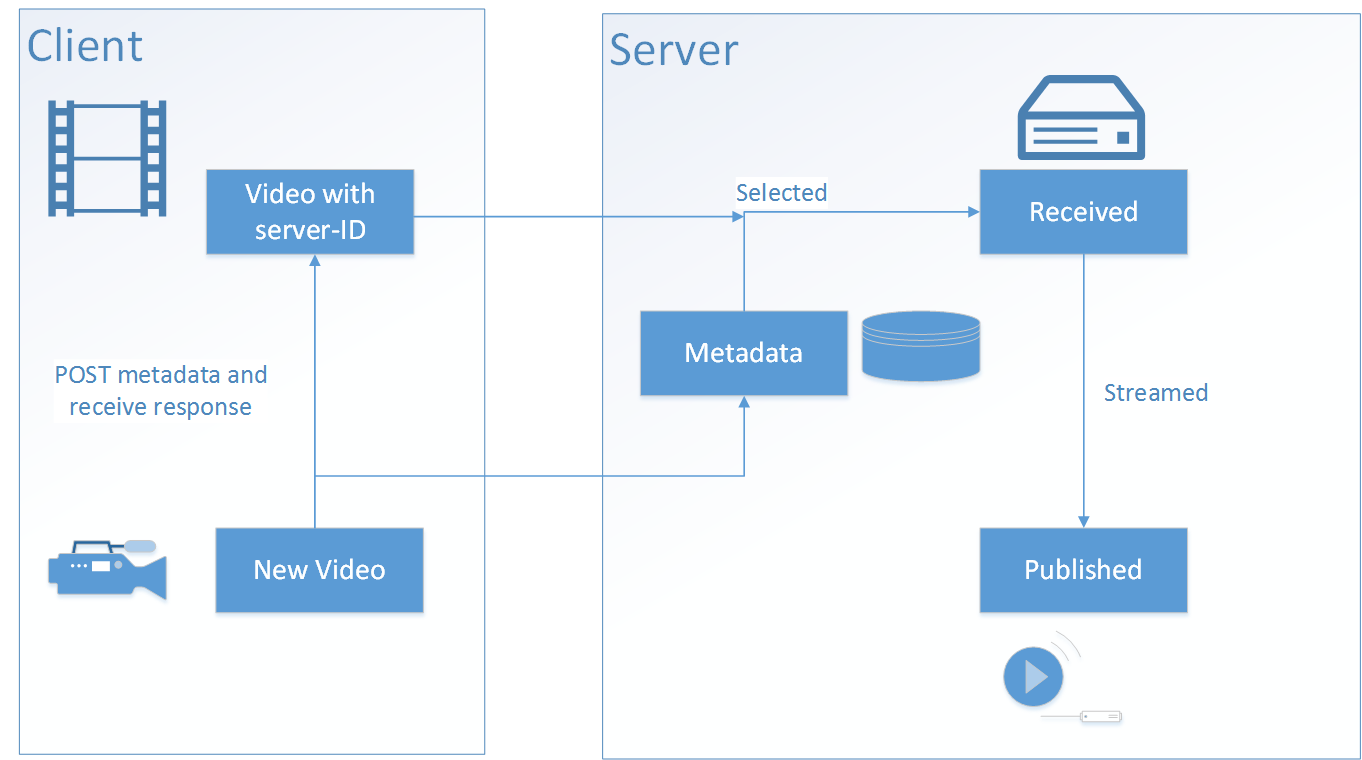
\includegraphics[width=\textwidth,height=\textheight,keepaspectratio]{video_states.png}
		\label{fig:states}
	\end{figure}
\end{frame}

\subsection{Selection algorithm}
\begin{frame}	
	\frametitle{Selection algorithm}
	\texttt{VideoRating} class assignes rank on metadata arrival
	Sigmoid transformation: $\forall x \in [shake, tilt]$
	\begin{align*}
		xs &= \cfrac{x^2}{15 * duration} \\
		f  &= \left(\cfrac{xs}{1+|xs|}\right)^3 &f  &\in [-1, 1] \\
		fn &= \cfrac{f + 1}{2}                  &fn &\in [0, 1]
	\end{align*}
	$$rating = 100 * \sqrt{ \sum\limits_{i \in sensors}{w_i m_i^2} },\ w_{shake} = 0.6,\ w_{tilt} = 0.4$$
	Selection process:
	\begin{itemize}
		\item Only videos starting after the last selected video ends are considered.
		\item Top-rated video is selected for upload
	\end{itemize}
\end{frame}

\begin{frame}	
	\frametitle{Selection algorithm (continued)}
	\begin{figure}[!t]
		\centering
		\subfloat[Scaling]{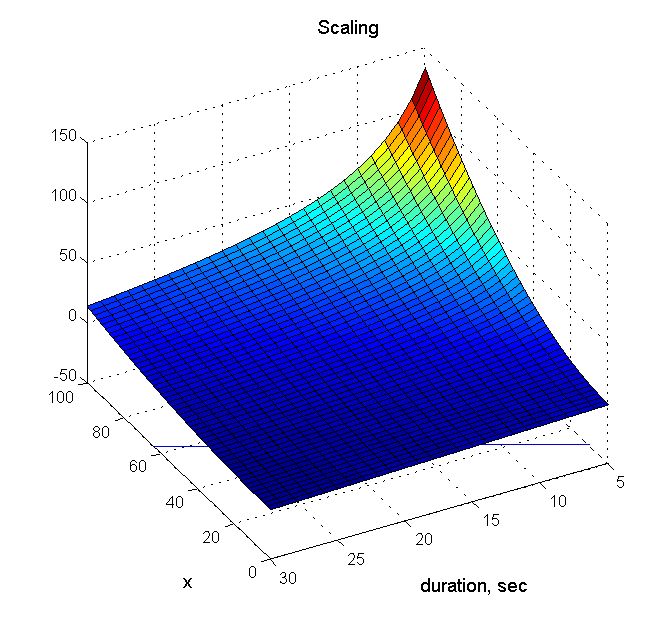
\includegraphics
			[width=.49\textwidth,height=.9\textheight,keepaspectratio]
			{scaling.png}%
			\label{fig:scaling}}
		\hfill
		\subfloat[Sigmoid transformation]{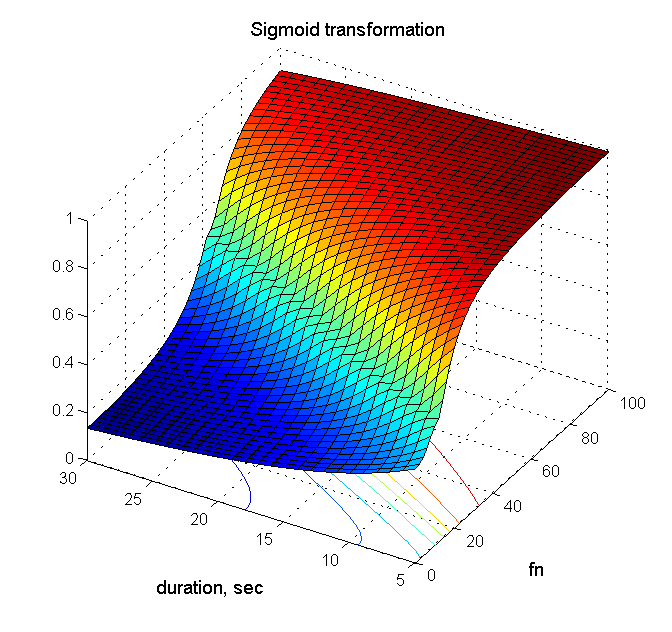
\includegraphics
			[width=.49\textwidth,height=.9\textheight,keepaspectratio]
			{sigmoid.png}%
			\label{fig:sigmoid}}
	\end{figure}
\end{frame}

\begin{frame}	
	\frametitle{Rating}
	\begin{figure}[!t]
		\centering
		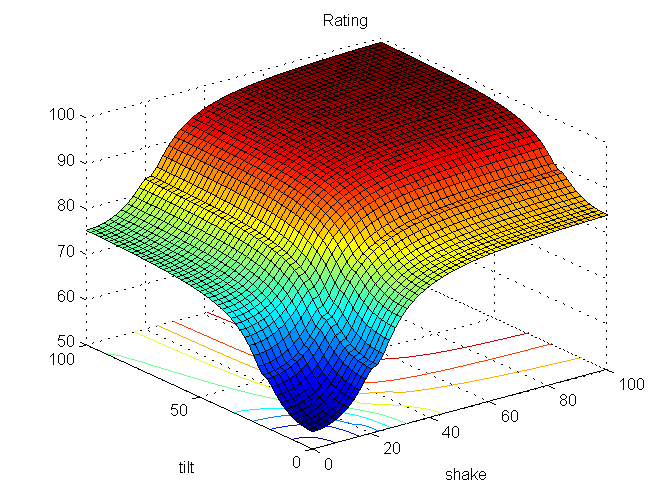
\includegraphics[width=\textwidth,height=.9\textheight,keepaspectratio]{rating.png}
		\label{fig:rating}
	\end{figure}
\end{frame}
	
\section{Teamwork}
\begin{frame}
	\frametitle{Teamwork}
	\begin{columns}[t]
		\begin{column}[t]{0.5\linewidth}
			Challenges:
			\begin{itemize}
				\item Distance
				\item Scheduling
				\item Parallel workload
				\item Late arrival of participants
				\item Limited means of communication
			\end{itemize}
		\end{column}
		\begin{column}[t]{0.5\linewidth}
			Technologies:
			\begin{itemize}
				\item Skype
				\item github.com
				\item Dropbox
			\end{itemize}
		\end{column}		
	\end{columns}
\end{frame}

\section{Conclusion}
\begin{frame}
	\frametitle{Demo}
		\begin{figure}[!t]
			\centering
			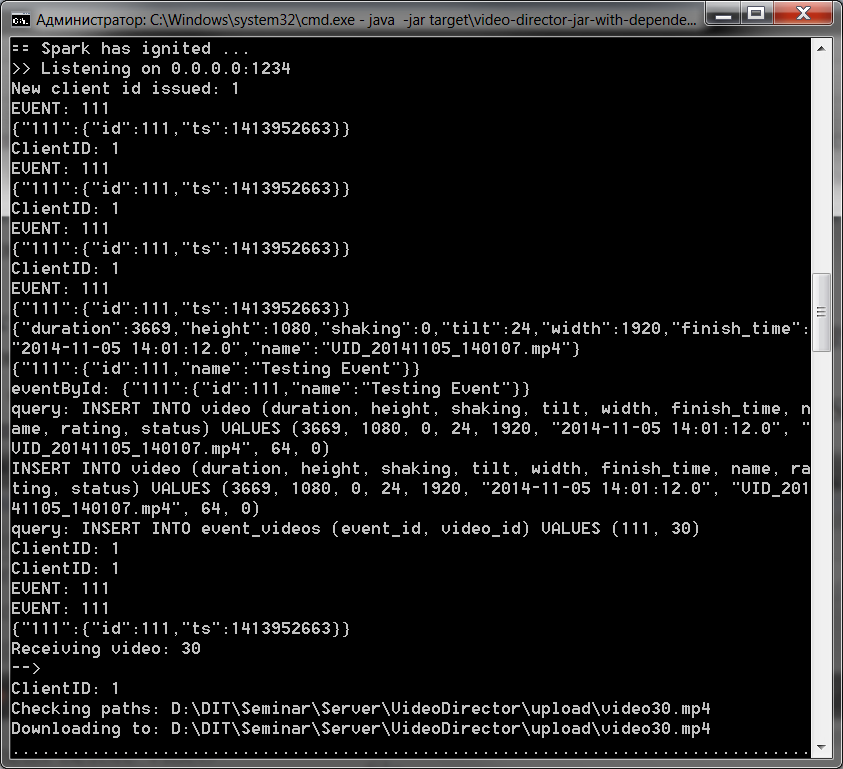
\includegraphics[width=\linewidth,height=.9\textheight,keepaspectratio]{server.png}
			\label{fig:server}
		\end{figure}
\end{frame}

\begin{frame}
	\frametitle{Future work}
	\begin{itemize}
		\item Web interface
		\item More sensors
		\item More sophisticated algorithm
		\item Synchronization
		\item Region of Interest
		\item Limited chunk size \& Streaming
	\end{itemize}
\end{frame}

\begin{frame}
	\frametitle{Conclusion}
	\begin{itemize}
		\item Client and server applications built
		\item Metadata format established
		\item Simple selection algorithm used
		\item Client and server can be tweaked to use other
		\begin{itemize}
			\item metadata formats
			\item sensors
			\item selection criteria
			\item selection algorithms
		\end{itemize}
	\end{itemize}
\end{frame}

\begin{frame}
	\frametitle{Questions}
	\centering
	\Huge Questions?
\end{frame}


%\begin{frame}
	%\frametitle{Frame 2}
	%\begin{itemize}
		%\item Four
		%\item Five
	%\end{itemize}
%\end{frame}
%
%\begin{frame}
	%\frametitle{Two Columns}
	%\begin{columns}[t]
		%\begin{column}[c]{5cm}
			%\footnotesize
			%\begin{tabular}[H]{|l||c|c|c|c|}
		        %\hline
		        %& \rotatebox{90}{Sugar } & \rotatebox{90}{Juicy } & \rotatebox{90}{Healthy } & \rotatebox{90}{Natural } \\
		        %\hline
		        %Fruit chews & $\times$ & $\times$ & & \\
		        %\hline
		        %Lollipop & $\times$ & & & \\
		        %\hline
		        %Chewing gum & & & $\times$ & \\
		        %\hline
		        %Fresh fruit & & $\times$ & $\times$ & $\times$ \\
		        %\hline
		    %\end{tabular}
		%\end{column}
		%\begin{column}[c]{5cm}
			%\usetikzlibrary{shapes.geometric}
			%\begin{tikzpicture}[thick,scale=0.7, every node/.style={transform shape}]
				%% [every node/.style={inner sep=0pt}]
				%\node (1) [circle, minimum size=18.75pt, fill=white, line width=0.625pt, draw=black] at (187.5pt, -75.0pt)  {};
				%\node (4) [circle, minimum size=18.75pt, fill=white, line width=0.625pt, draw=black] at (187.5pt, -225.0pt)  {};
				%\node (2) [circle, minimum size=18.75pt, fill=white, line width=0.625pt, draw=black] at (150.0pt, -150.0pt)  {};
				%\node (3) [circle, minimum size=18.75pt, fill=white, line width=0.625pt, draw=black] at (225.0pt, -150.0pt)  {};
				%\draw [line width=0.625, color=black] (2) to  (1);
				%\draw [line width=0.625, color=black] (3) to  (1);
				%\draw [line width=0.625, color=black] (4) to  (2);
				%\node at (187.5pt, -57.5pt) {\textcolor{black}{Fresh fruit}};
				%\node at (187.5pt, -242.5pt) {\textcolor{black}{Lolipop}};
				%\node at (113.75pt, -150.0pt) {\textcolor{black}{Fruit chew}};
				%\node at (268.25pt, -150.0pt) {\textcolor{black}{Chewing gum}};
			%\end{tikzpicture}
		%\end{column}
	%\end{columns}
%\end{frame}

\end{document}
